%!TEX root = pyconuk2016.tex

\blankscreen{
        Entity Paradigm\textCR
}

\begin{frame}{The Entity Paradigm}

    \tikzstyle{primary} = [
        rectangle, rounded corners, line width=0.4mm, draw=blue,
        minimum height=2cm, minimum width=3cm, text width=3cm
    ]
    \tikzstyle{substance} = [
        rectangle, rounded corners, line width=0.4mm, draw=blue,
        top color=white, bottom color=blue!20,
        minimum height=2cm, minimum width=3cm
    ]
    \tikzstyle{attribute} = [
        rectangle, rounded corners, line width=0.4mm, draw=red,
        minimum width=2cm, fill=white, opacity=1
    ]
    \tikzstyle{hidden} = [
        rectangle, rounded corners,
        % line width=0.4mm, draw=green,
        minimum height=3cm, minimum width=6cm
    ]
    \tikzstyle{real} = [rectangle]
    \tikzstyle{line} = [line width=0.5mm]

    \begin{center}
        \resizebox{10cm}{!}{
            \begin{tikzpicture}
                \node[hidden](1) at (0, 9) {};
                    \node[hidden](2) at (-3, 6){};
                        \node[hidden](3) at (-3, 3){};
                            \node[hidden](4) at (-3, 0){};

                    \node[hidden](5) at (3, 6){};
                        \node[hidden](6) at (3, 3){};
                            \node[hidden](7) at (3, 0){};

                \node[hidden](8) at (9, 9){};
                    \node[hidden](9) at (9, 6){};
                        \node[hidden](10) at (9, 3){};
                            \node[hidden](11) at (9, 0){};


                \node(real_mx5)[real] at (4){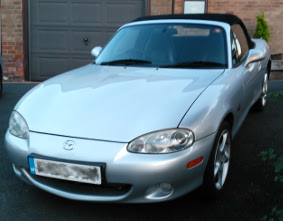
\includegraphics[width=3cm]{images/mx5}};

                \node(real_mondeo)[real] at (7){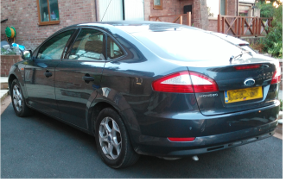
\includegraphics[width=3cm]{images/mondeo}};

                \node(my_mx5) at (3)[primary]{My\\ Toy Car};
                \draw(real_mx5.north)--(my_mx5.south);

                \node(my_mondeo) at (6)[primary]{My\\  Big Car};
                \draw(real_mondeo.north) -- (my_mondeo.south);

                \node(silver)[attribute] at (my_mx5.east){Silver};
                \node(abc123)[attribute, anchor=north west] at (silver.south west){ABC 123};

                \node(grey)[attribute] at (my_mondeo.east){Grey};
                \node(xyz789)[attribute, anchor=north west] at (grey.south west){XYZ 789};

                \node(mx5) at (2)[substance]{Mazda MX5};
                \draw(my_mx5.north) -- (mx5.south);

                \node(mondeo) at (5)[substance]{Ford Mondeo};
                \draw(my_mondeo.north) -- (mondeo.south);

                \node(car) at (1)[substance]{Car};
                \draw(mx5.north) -- (car.south);
                \draw(mondeo.north) -- (car.south);

            \end{tikzpicture}
        }
    \end{center}

\end{frame}

\begin{frame}{The Entity Paradigm}

    \tikzstyle{primary} = [
        rectangle, rounded corners, line width=0.4mm, draw=blue,
        minimum height=2cm, minimum width=3cm, text width=3cm
    ]
    \tikzstyle{substance} = [
        rectangle, rounded corners, line width=0.4mm, draw=blue,
        top color=white, bottom color=blue!20,
        minimum height=2cm, minimum width=3cm
    ]
    \tikzstyle{attribute} = [
        rectangle, rounded corners, line width=0.4mm, draw=red,
        minimum width=2cm, fill=white, opacity=1
    ]
    \tikzstyle{hidden} = [
        rectangle, rounded corners,
        % line width=0.4mm, draw=green,
        minimum height=3cm, minimum width=6cm
    ]
    \tikzstyle{real} = [rectangle]
    \tikzstyle{line} = [line width=0.5mm]

    \begin{center}
        \resizebox{10cm}{!}{
            \begin{tikzpicture}
                \node[hidden](1) at (0, 9) {};
                    \node[hidden](2) at (-3, 6){};
                        \node[hidden](3) at (-3, 4.5){};
                            \node[hidden](4) at (-3, 0){};

                    \node[hidden](5) at (3, 6){};
                        \node[hidden](6) at (3, 4.5){};
                            \node[hidden](7) at (3, 0){};

                \node[hidden](8) at (9, 9){};
                    \node[hidden](9) at (9, 6){};
                        \node[hidden](10) at (9, 3){};
                            \node[hidden](11) at (9, 0){};


                \node<1->(real_mx5)[real] at (4){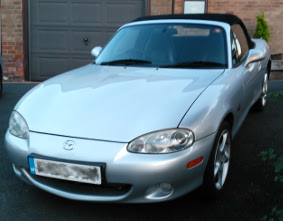
\includegraphics[width=3cm]{images/mx5}};
                \node(real_mondeo)[real] at (7){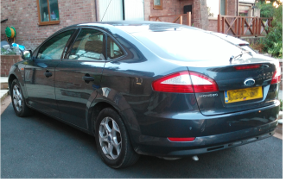
\includegraphics[width=3cm]{images/mondeo}};

                \node<1->(my_mx5) at (3)[primary]{My\\ Toy Car};
                \draw<1->(real_mx5.north)--(my_mx5.south);

                \node<1->(my_mondeo) at (6)[primary]{My\\  Big Car};
                \draw<1->(real_mondeo.north) -- (my_mondeo.south);

                \node<1->(silver)[attribute] at (my_mx5.east){Silver};
                \node<1->(abc123)[attribute, anchor=north west] at (silver.south west){ABC 123};

                \node<1->(grey)[attribute] at (my_mondeo.east){Grey};
                \node<1->(xyz789)[attribute, anchor=north west] at (grey.south west){XYZ 789};

                \node<1->(car) at (1)[substance]{Car};
                \draw<1->(my_mx5.north) -- (car.south);
                \draw<1->(my_mondeo.north) -- (car.south);

                \node<2->(mx5_attr)[attribute, anchor=north west] at (abc123.south west) {Mazda MX5};
                \node<2->(mondeo_attr)[attribute, anchor=north west] at (xyz789.south west) {Ford Mondeo};

            \end{tikzpicture}
        }
    \end{center}

\end{frame}
